\documentclass{article}
\usepackage[utf8]{inputenc}
\usepackage[T1]{fontenc}
\usepackage{graphicx}
\usepackage{hyperref}
\usepackage{geometry}
\geometry{margin=1in}

\title{AMHAN}
\date{Encyclopaedia Britannica (1771)}

\begin{document}
\maketitle

\section*{Historical source}
\textbf{Entry ID:} \texttt{entry-amhan-560} \\
\textbf{Volume ID:} 191253801 \\
\textbf{Character Count:} 507

\subsection*{Extracted Text}
AMHAN, or AVARA, a province of Anything, field to extend so leagues from raft in welf. It is considered as the most noble in the whole empire, both on account of its being the ideal reference of the A- bythnis monuments, and among a particular dialect different from all the craft, which by reason of the emperor being brought up in the previous works because the language of the course and of the police people. Here is the famed rock Amba-gelthen, where the young morachs were formerly confined. See AvaA.



\section*{Source record}
\begin{itemize}
\item \textbf{Dataset:} \texttt{NationalLibraryOfScotland/encyclopaedia\_britannica\_illustrated}
\item \textbf{Dataset Revision:} \texttt{309f765b1ecc83e0a7f7762e44b4a927a7555443}
\item \textbf{Page ID:} \texttt{britannica:309f765b1ecc83e0a7f7762e44b4a927a7555443:train:560} \\
  \textbf{Filename:} \texttt{page-0560-c458f594fc79.jpg} \\
  \textbf{Row Index:} 560 \\
  \textbf{SHA256:} \texttt{c458f594fc79392e...}
\end{itemize}

\begin{figure}[h]
\centering
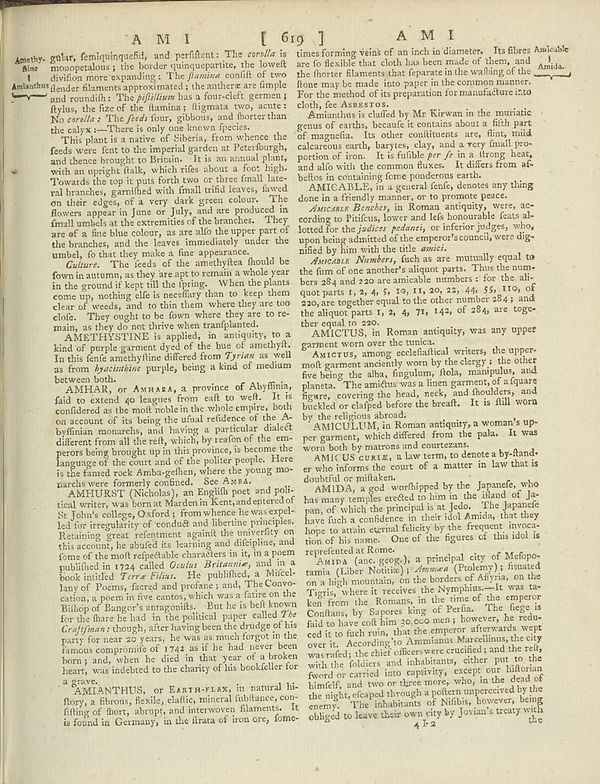
\includegraphics[width=0.85\textwidth]{../scans/page-0560-c458f594fc79.jpg}
\caption*{Source scan: \texttt{page-0560-c458f594fc79.jpg}}
\end{figure}

\end{document}
